\def\Version{0.1}
\documentclass{article}
\usepackage[margin = 2cm]{geometry}
\usepackage[english]{babel}
\usepackage[utf8]{inputenc}
\usepackage[T1]{fontenc}
\usepackage{xcolor}
\usepackage{booktabs}
\usepackage{acronym}
\usepackage{listings}
\usepackage[hidelinks]{hyperref}
\usepackage{amsthm}
\usepackage{graphicx}
\theoremstyle{definition}
\newtheorem{example}{Example}[section]
\graphicspath{{../Images/}}

\usepackage{tikz} % ------------------------------- %
\usetikzlibrary{arrows}								%
\usetikzlibrary{calc}								%
\usetikzlibrary{decorations.footprints}				%
\usetikzlibrary{decorations.pathmorphing}			%
\usetikzlibrary{decorations.text}					%
\usetikzlibrary{fadings}							%
\usetikzlibrary{fit}								%
\usetikzlibrary{intersections}						%
\usetikzlibrary{matrix}								%
\usetikzlibrary{mindmap}							%
\usetikzlibrary{patterns}							%
\usetikzlibrary{plotmarks}							%
\usetikzlibrary{positioning}						%
\usetikzlibrary{shadows}							%
\usetikzlibrary{shapes.geometric}					%
\usetikzlibrary{shapes}								%
\usetikzlibrary{trees}								%
\usepackage{pgfplots}								%
\usepackage{pgfpages}								%
\pgfplotsset{compat=newest} % --------------------- %

\tikzstyle{block} = [draw, fill=green!50!cyan!15, rectangle, minimum height=3em, minimum width=4.5em, node distance=8em]
\tikzstyle{file} = [draw, fill=orange!50!yellow!15, rectangle, node distance=5em]
\tikzstyle{cloud} = [draw, fill=gray!20, ellipse, minimum height=3em, minimum width=4.5em, node distance=8em]

\newcommand{\itemheader}[1]{\item \textbf{#1}}
\lstset{basicstyle=\ttfamily}

%
\title{The CITE App Manual}
\date{Version \Version}
\author{Beagle Boys\footnote{The research leading to these results has received funding from the European Community through the Erasmus+ project 2019-1-NO01-KA203-060257 ``Face It'', and from Lule{\aa} University of Technology, Uppsala University and the Norwegian University of Science and Technology through a series of local pedagogical development projects.}}
%
\begin{document}
\maketitle
\tableofcontents
\newpage

\section*{Acronyms}
\begin{acronym}
	\acro{CDIO}			[CDIO]	{Conceiving, Designing, Implementing, and Operating}
	\acro{ILO}			[ILO]	{Intended Learning Outcome}
	\acro{ITS}			[ITS]	{Intelligent Tutoring System}
	\acro{KCG}			[KCG]	{Knowledge Components Graph}
	\acro{KCM}			[KCM]	{Knowledge Components Matrix}
	\acroplural{KCM}	[KCMs]	{Knowledge Components Matrices}
	\acro{KC}			[KC]	{Knowledge Component}
	\acro{LMS}			[LMS]	{Learning Management System}
	\acro{LTU}			[LTU]	{Lule{\aa} University of Technology}
	\acro{NTNU}			[NTNU]	{Norwegian University of Science and Technology}
	\acro{PLO}			[PLO]	{Program Learning Outcome}
	\acro{SOLO}			[SOLO]	{Structure of Observed Learning Outcomes}
	\acro{TLA}			[TLA]	{Teaching and Learning Activity}
	\acroplural{TLA}	[TLAs]	{Teaching and Learning Activities}
	\acro{UU}			[UU]	{Uppsala University}
\end{acronym}
\newpage

\section{What is this? And why should I use it?}
\label{sec:what_is_this_and_why_should_i_use_it}

Among the needs of the persons involved in higher education, we identified the following:
%
\begin{description}
	\item[for students:] when studying, have a clear idea of how courses connect to each other from a contents-wise perspective, and of why it is important to memorize and understand what it is being asked to study (e.g., why shall I understand what is the geometrical interpretation of eigenvalues?);
	\item[for teachers:] when modifying the contents of the own courses, have a holistic view on the effects of these contents modifications on the program (e.g., if I won't teach this concept anymore in my course, how will this affect the following courses?);
	\item[for program boards:] when modifying the structure of a program, have instruments that help steering discussions and taking decisions based on evidence instead of opinions (e.g., why shall this course be taught before that other one?);
	\item[for administrators:] when inspecting and assessing the program quality, have instruments that are quantitative oriented, explainable, and communicable, so to ease discussions and reporting.
\end{description}

\begin{centering}
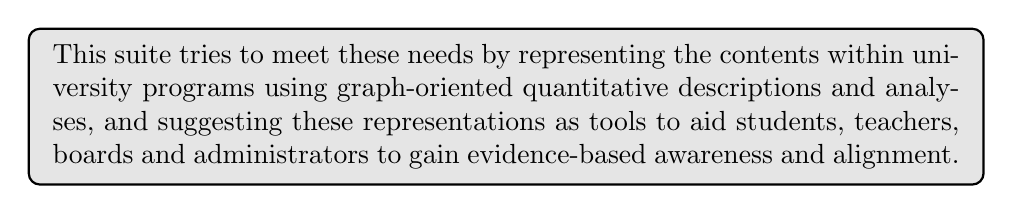
\begin{tikzpicture}
\node [minimum width = \textwidth, rounded corners, draw, thick, fill = black!10!white, align = justify, text width = 0.95\textwidth, inner sep = 0.2cm]
{This suite tries to meet these needs by representing the contents within university programs using graph-oriented quantitative descriptions and analyses, and suggesting these representations as tools to aid students, teachers, boards and administrators to gain evidence-based awareness and alignment.};
\end{tikzpicture}
\end{centering}

The approach is the following: 
\begin{enumerate}
	\item consider courses and programs as opportune flows and transformations of prerequisite contents-wise knowledge (expressed in terms of prerequisite concepts) into developed contents-wise knowledge (expressed in terms of \acp{KC}. See Section~\ref{sec:lexicon} for an explanation of all the various terms); 
	\item analyze and visualize the structure of a program (or a part of it) in terms of these concepts development flows;
	\item connect these concept development flows to the \acp{TLA}, \acp{ILO}, and \acp{PLO} of the various courses and the whole program;
	\item increase the awareness of the stakeholders by visualizing and analysing these connections and flows in (hopefully) self-explanatory ways.
\end{enumerate}

\begin{example}
	%
	To exemplify this process, assume that the contents of the fictitious ``\emph{Course X}'' can be expressed in terms of which prerequisite concepts are required by the students plus which concepts are developed in the course itself. E.g., let the prerequisites and developed concepts be:
	%
	\begin{itemize}
		\item prerequisites: ``\emph{vector spaces}'', ``\emph{linearity}'', and ``\emph{matrices-vectors multiplication}'';
		\item developed: ``\emph{eigenvalues}'', ``\emph{characteristic polynomials}'', ``\emph{computation of Jordan forms}''.
	\end{itemize}
	%
	Ideally (and as an example), the teacher knows that the developed concepts are ideally reached by building on the prerequisite ones as summarized as in Figure~\ref{fig:KCM}. I.e.,
	%
	\begin{itemize}
		\item to be able to learn about \emph{eigenvalues} students should ideally have a prerequisite learning level (using Bloom's taxonomy~\cite{bloom1956taxonomy} as an illustrative example) \emph{2 - understand} for both prerequisite concepts \emph{vector spaces} and \emph{linearity};
		\item to be able to learn about \emph{characteristic polynomials} students should ideally have a prerequisite learning level \emph{2 - understand} about \emph{matrices and vectors multiplication}, and have reached - while studying for \emph{Course X} - a learning level \emph{1 - remember} about the developed concept \emph{eigenvalues};
		\item to be able to learn about \emph{computation of Jordan forms} students should ideally have a prerequisite learning level \emph{1 - remember} for the prerequisite \emph{linearity} and level \emph{2 - understand} about the developed \emph{eigenvalues} and \emph{characteristic polynomials}.
	\end{itemize}
	%
	\begin{figure}[!htbp]
		\centering
		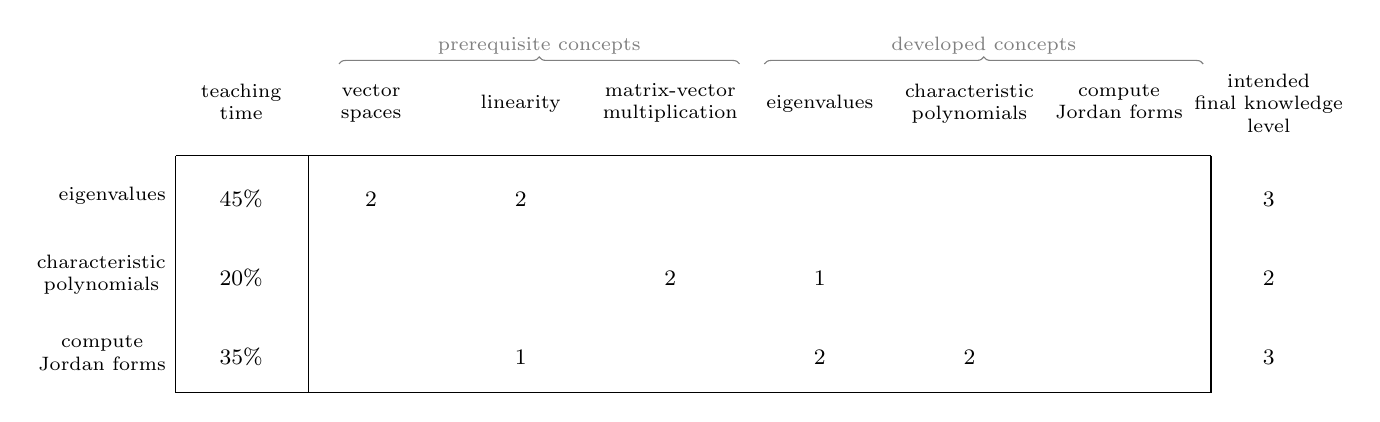
\begin{tikzpicture}
[
	Concept/.style	= {font = \scriptsize, align = center, anchor = base, minimum height = 1cm},
	row sep			= {1cm,between origins},
	column sep		= {1.9cm,between origins},
	column 1/.style	= {column sep = 1cm, nodes = {fill = black!00!white}, },
]

	\matrix (M)
	[
		matrix of nodes,
		nodes					= {font = \footnotesize, inner sep = 0cm, text height = 0.3cm, text width = 0.65cm, align = center, anchor = base},
		nodes in empty cells	= true,
	]
	{
		45\%  & 2 & 2 &   &   &   &   & 3 \\
		20\%  &   &   & 2 & 1 &   &   & 2 \\
		35\%  &   & 1 &   & 2 & 2 &   & 3 \\
	};

	\node (p0) [Concept, above = 0.5cm of M-1-1, minimum width = 1.7cm] {teaching \\ \phantom{g} time \phantom{g}};
	\node (p1) [Concept, above = 0.5cm of M-1-2] {vector \\ spaces};
	\node (p2) [Concept, above = 0.5cm of M-1-3] {linearity};
	\node (p3) [Concept, above = 0.5cm of M-1-4] {matrix-vector \\ multiplication};
	%
	\node (p4) [Concept, above = 0.5cm of M-1-5] {eigenvalues};
	\node (p5) [Concept, above = 0.5cm of M-1-6] {characteristic \\ polynomials};
	\node (p6) [Concept, above = 0.5cm of M-1-7] {compute \\ \phantom{g} Jordan forms \phantom{g}};
	%
	\node (p7) [Concept, above = 0.5cm of M-1-8, minimum width = 1.7cm] {intended \\ final knowledge \\ level};
	%
	\node (c1) [Concept, left = 0.5cm of M-1-1] {eigenvalues};
	\node (c2) [Concept, left = 0.5cm of M-2-1] {characteristic \\ polynomials};
	\node (c3) [Concept, left = 0.5cm of M-3-1] {compute \\ Jordan forms};

	\node (auxA) [coordinate, above = 0.5cm of p1.west, xshift = +0.1cm] {};
	\node (auxB) [coordinate, above = 0.5cm of p3.east, xshift = -0.1cm] {};
	\node (auxC) [coordinate, above = 0.5cm of p4.west, xshift = +0.1cm] {};
	\node (auxD) [coordinate, above = 0.5cm of p6.east, xshift = -0.1cm] {};
	%
	\draw [decorate, decoration = brace, draw = black!50!white] (auxA) -- (auxB) node [above, pos = 0.5, font = \scriptsize, text = black!50!white] {prerequisite concepts};
	%
	\draw [decorate, decoration = brace, draw = black!50!white] (auxC) -- (auxD) node [above, pos = 0.5, font = \scriptsize, text = black!50!white] {developed concepts};

	% auxiliary nodes to draw the matrix
	\node (MM11) [coordinate] at (c1.north east) {};
	\node (MM21) [coordinate] at (c3.south east) {};
	\node (MM12) [coordinate] at ($(p0.north east)!(c1.north east)!(p0.south east)$) {};
	\node (MM22) [coordinate] at ($(p0.north east)!(c3.south east)!(p0.south east)$) {};
	\node (MM13) [coordinate] at ($(p6.north east)!(c1.north east)!(p6.south east)$) {};
	\node (MM23) [coordinate] at ($(p6.north east)!(c3.south east)!(p6.south east)$) {};

	\draw [solid] (MM11) -- (MM21);
	\draw [solid] (MM21) -- (MM23);
	\draw [solid] (MM23) -- (MM13);
	\draw [solid] (MM13) -- (MM11);
	\draw [solid] (MM12) -- (MM22);

\end{tikzpicture}


		\caption{Tabular representation of how \emph{Course X}'s developed concepts are ideally reached by building on its prerequisites. In this document we call this matrix a \acf{KCM}.}
		\label{fig:KCM}
	\end{figure}
	%
	The \ac{KCM} in Figure~\ref{fig:KCM} can be converted into its graph representation defined in Figure~\ref{fig:KCG}.
	%
	\begin{figure}[!htbp]
		\centering
		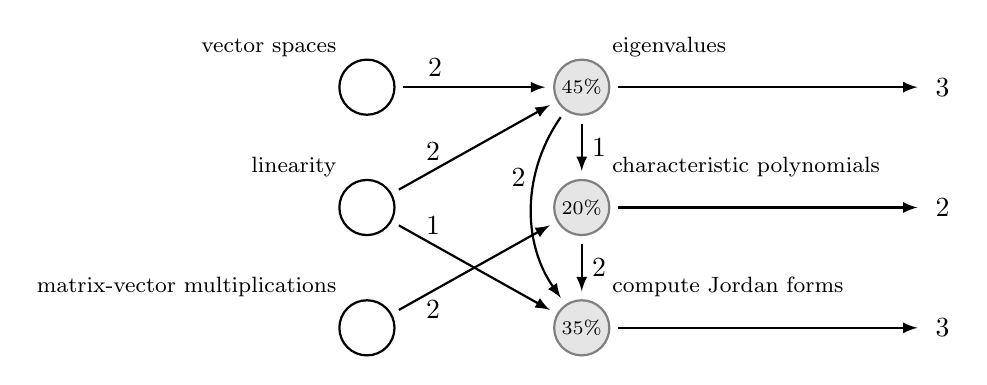
\begin{tikzpicture}
[
	ILO/.style	= {circle, draw = black!50!white, fill = black!10!white, minimum size = 0.7cm, inner sep = 0cm, font = \scriptsize},
	pre/.style	= {ILO, draw = black, fill = white},
	comment/.style	= {font = \footnotesize},
	node distance = 0.8cm and 0.8cm,
	every path/.style = {-latex, thick, shorten < = 0.1cm, shorten > = 0.1cm},
]

	\node (pre1) [pre] {};
	\node (pre2) [pre, below = of pre1] {};
	\node (pre3) [pre, below = of pre2] {};
	%
	\node (ILO1) [ILO, right = 2cm of pre1] {45\%};
	\node (ILO2) [ILO, below = of ILO1] {20\%};
	\node (ILO3) [ILO, below = of ILO2] {35\%};
	%
	\node (aux1) [coordinate, right = 4cm of ILO1] {};
	\node (aux2) [coordinate, right = 4cm of ILO2] {};
	\node (aux3) [coordinate, right = 4cm of ILO3] {};

	\node [comment, above left = 0cm of pre1] {vector spaces};
	\node [comment, above left = 0cm of pre2] {linearity};
	\node [comment, above left = 0cm of pre3] {matrix-vector multiplications};
	%
	\node [comment, above right = 0cm of ILO1] {eigenvalues};
	\node [comment, above right = 0cm of ILO2] {characteristic polynomials};
	\node [comment, above right = 0cm of ILO3] {compute Jordan forms};

	\draw (pre1) -- (ILO1) node [pos = 0.25, above] {2};
	\draw (pre2) -- (ILO1) node [pos = 0.25, above] {2};
	\draw (pre2) -- (ILO3) node [pos = 0.25, above] {1};
	\draw (pre3) -- (ILO2) node [pos = 0.25, below] {2};

	\draw (ILO1) -- (ILO2) node [pos = 0.5, right] {1};
	\draw [out = 235, in = 125] (ILO1) to node [pos = 0.35, left] {2} (ILO3);
	\draw (ILO2) -- (ILO3) node [pos = 0.5, right] {2};

	\draw (ILO1) -- (aux1) node [pos = 1.0, right] {3};
	\draw (ILO2) -- (aux2) node [pos = 1.0, right] {2};
	\draw (ILO3) -- (aux3) node [pos = 1.0, right] {3};


\end{tikzpicture}

		\caption{Graphical representation of the \acf{KCM} in Figure~\ref{fig:KCM} as a (as called in this document) \acf{KCG}.}
		\label{fig:KCG}
	\end{figure}
	%
	Within a program, the concepts developed in some courses may be prerequisites for other courses. This means that one can join the various individual \acp{KCM} and \acp{KCG} into a program-wide representation. This operation produces a directed graph representing the various ``\emph{concepts learning flows}'' that students ideally follow during their studies. 
	%
\label{exa:KCM}
\end{example}

\ac{KCG} representations can help meeting the stakeholders' needs listed at the beginning as follows:
%
\begin{description}
	\item[for teachers:] changing the content of a course means changing the learning flows in the \ac{KCG}. With the here proposed software one may then check if course modifications (i.e., \ac{KCM} modifications) will lead to broken, redundant or non-pedagogically ideal paths in the \ac{KCG};
	\item[for program boards:] the same software may be used to manage the discussions during boards meetings, and be a digital canvas where to test the meaningfulness of different program changes. This may help taking an evidence-based approach to designing and modifying programs;
	\item[for students:] the software may be used by students to get intuitions about the purpose of studying specific concepts, what is the effect of having forgotten parts of the program, plus how central each part is within the program flow. The software may thus help single students perform self-assessment and monitoring, and help gaining holistic viewpoints on the expected learning process;
	\item[for quality assurance personnel:] the software may be used also by quality assurance to perform automatic assessments of structural properties of the programs. We envision to use these representations also to help performing comparisons of different programs in different institutions - however we still did not implement these features.
\end{description}



\subsection{What if I just want to analyse a single course?}

The software may be used by a teacher or set of teachers also in the context of a \emph{single course}. In other words, in the following one may build up a \ac{KCM} for each \emph{individual class} instead of for each \emph{individual course}. This means that this software may be used as it is also for planning, visualizing, assessing and discussing the detailed contents of a course, instead of a program or part of it.



\section{An overview of the structure of this manual}
\label{sec:an_overview_of_the_structure_of_this_manual}

The first part of the manual aims to explain how to use the software.

\begin{description}

\item[Section~\ref{sec:what_is_this_and_why_should_i_use_it}] describes the
	general purpose of the software, and frames the bigger picture;

\item[Section~\ref{sec:inserting_the_data}] describes how to collect and
	insert the data that is processed by the software;

\item[Section~\ref{sec:analysing_the_data}] describes how to use the
	software to produce information;

\item[Section~\ref{sec:interpreting_the_results}] describes how to interpret
	that information.

\end{description}


The appendix explains what the various things mean. % Should be reworded to better reflect the meaning.

\begin{description}

\item[Section~\ref{sec:lexicon}] is a glossary of the terms that are used
	throughout the manual; 

\item[Section~\ref{sec:how_to_define_the_knowledge_components_list}] is not
	yet implemented. It should describe how to identify and define the
	\acp{KC}. This section is ancillary to
	Section~\ref{sec:inserting_the_data};

\item[Section~\ref{sec:how_to_interpret_and_assign_taxonomy_levels}] is not
	yet implemented. It should describe how to interpret (and thus
	assign) knowledge taxonomy levels. Also this section is
	ancillary to Section~\ref{sec:inserting_the_data};

\item[Section~\ref{sec:how_to_identify_ilo}] is not yet implemented. It
	should describe how to identify and define the \acp{ILO}. Also this
	section is ancillary to
	Section~\ref{sec:inserting_the_data};

\item[Section~\ref{sec:how_to_identify_tla}] is not yet implemented. It
	should have the same purpose has the above item, and is dedicated to
	defining the \acp{TLA}. Also this section is ancillary to
	Section~\ref{sec:inserting_the_data};

\item[Section~\ref{sec:debugging}] collects a series of known bugs /
	non-ideal features in the software that may make Matlab stop
	running. Please consider that this software is more in
	alpha-testing than in beta-testing.

\end{description}


\section{Inserting the data}
\label{sec:inserting_the_data}

The purpose of the software is to create graphical representations of the
programs. The software suite works by merging independent information from
different courses. More specifically, the following items are required:
%
\begin{enumerate}
\item a \ac{KCM} (which is a specialized spreadsheet file) for each course;
\item a ``\emph{program definition file}'' (which is a plain text file) that
	indicates which \acp{KCM} are included in the program.
\end{enumerate}
%
This section goes over the procedure for creating the files above, and for
how to enter information in them.

\subsection{Creating the database containing the files above}
\label{creating_the_database}

The first step is to create a database containing the \ac{KCM} spreadsheets
and the program definition file. The \acp{KCM} may be in a remote location,
such as on Google Drive or Dropbox, or on the computer that runs this
software. The program definition file must be available on the computer,
regardless of where the \acp{KCM} are located.

\textbf{As for the program definition file}, it must be a tabulated list
structured as in Table~\ref{tab:progexample}. This means that the first row
\emph{must} be identical to that of the first row in
Table~\ref{tab:progexample}, where each column is separated by exactly one
tab. The other rows should each have a course code, a version number (any
positive rational number is valid) and a link to a \ac{KCM} on a remote
location (Google Drive, Dropbox, etc.), in order. Also here, each column has
to be separated by exactly one tab. 

\begin{table}[!htbp]
	\centering
	\caption{Example of a program definition file. Each column has to be
	separated by exactly one tab (this means that the columns may not
	look like ``aligned'' in the file).}
	\label{tab:progexample}
	\ttfamily
	\begin{tabular}[t]{lll}
		\toprule
			coursecode & version & link \\
		\midrule
			TX8101 & 2 & (URL link to the spreadsheet file) \\
			AF9101 & 3 & (URL link to the spreadsheet file) \\
			XY0011 & 2 & (URL link to the spreadsheet file) \\
		\bottomrule
	\end{tabular}
\end{table}

This file, let's call it \texttt{my-program-definition-file.txt}, should be
located in a specific path. To understand where, consider the base folder
shown and described in Figure~\ref{fig:file-structure-base-folder}.

\begin{figure}[!htbp]
	\centering
	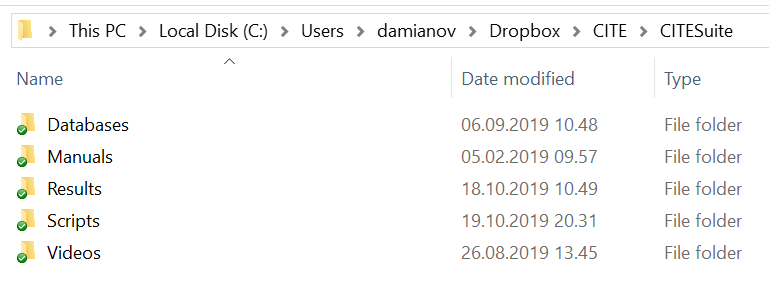
\includegraphics{file-structure-base-folder} 
	% TODO Get a new figure in place where it says ``COnCUR''.
	\caption{Structure of the base folder: when extracting the downloaded \texttt{COnCUR.zip} file, you obtain this.}
	\label{fig:file-structure-base-folder}
\end{figure}

From the base folder in Figure~\ref{fig:file-structure-base-folder}, enter
the ``Databases'' folder. The folder should be structured as in
Figure~\ref{fig:file-structure-databases-folder}.

\begin{figure}[!htbp]
	\centering
	% TODO Ibidem.
	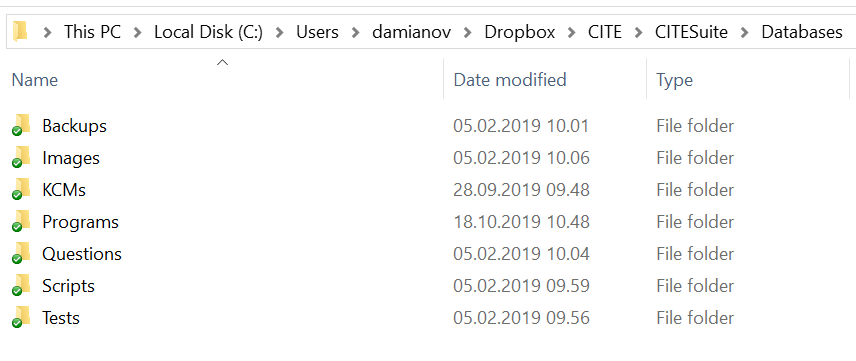
\includegraphics{file-structure-databases-folder}
	\caption{Structure of the ``databases'' folder.}
	\label{fig:file-structure-databases-folder}
\end{figure}

The \texttt{my-program-definition-file.txt} goes inside the folder
``Programs''. \textbf{As an example,} a person that has a few program
definition files may have a situation like in
Figure~\ref{fig:file-structure-programs-folder}.

\begin{figure}[!htbp]
	\centering
	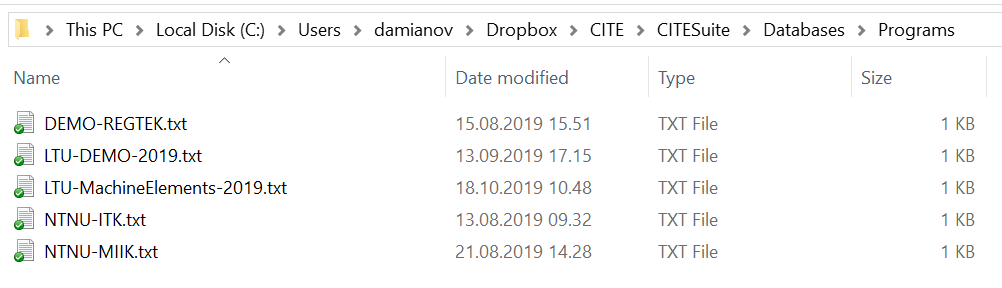
\includegraphics{file-structure-programs-folder}
	\caption{Example of how the ``Programs'' folder may look like. Note
	that when downloading the software suite you get an almost empty
	Programs folder (except a demo file).}
	\label{fig:file-structure-programs-folder}
\end{figure}

As for the \acp{KCM}, they can be either on the Internet or on a local
folder. Sections~\ref{sec:dbinternet}~and~\ref{sec:dblocal} explain how to
structure these.


\subsubsection{Internet-based case}
\label{sec:dbinternet}

One may want to keep the \ac{KCM} files on the Internet, so that different
persons may access and/or edit the information in an asynchronous way. The
program definition file tells where these are, and the software works by
downloading the \acp{KCM} when one runs the analysis. The structure of the
Internet-based database of the \acp{KCM} is as in
Figure~\ref{fig:dbinternet}.

\begin{figure}[!htbp]
	\centering
	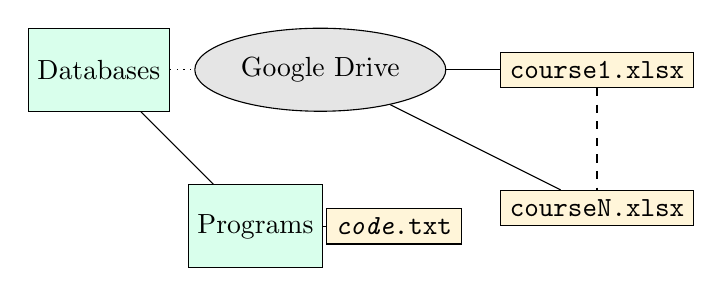
\begin{tikzpicture}[auto]
		\node [block, name=root] {Databases};
		\node [block, name=programs, below right of=root] {Programs};
		\node [file, name=pfile, right of=programs] {\texttt{\textit{code}.txt}};
		\node [cloud, name=drive, right of=root] {Google Drive};
		\node [file, name=sheet1, right of=drive, node distance=10em] {\texttt{course1.xlsx}};
		\node [file, name=sheetN, below of=sheet1] {\texttt{courseN.xlsx}};
		
		\draw [draw] (root) -- (programs);
		\draw [draw, dotted] (root) -- (drive);
		\draw [draw] (programs) -- (pfile);
		\draw [draw] (drive) -- (sheet1);
		\draw [draw] (drive) -- (sheetN);
		\draw [draw, dashed] (sheet1) -- (sheetN);
	\end{tikzpicture}
	\caption{Diagram of the internet-based program database.}
	\label{fig:dbinternet}
\end{figure}

This means that the program definition file should be placed in the
\texttt{Programs} folder of the \texttt{Databases} folder, as said before,
and the links that it contains should point to the corresponding \acp{KCM}.

\subsubsection{Local repository case}
\label{sec:dblocal}

The other option is to have the \ac{KCM} files placed in suitable folders.
The structure of such a database is given in Figure~\ref{fig:dblocal}.

\begin{figure}[!htbp]
	\centering
	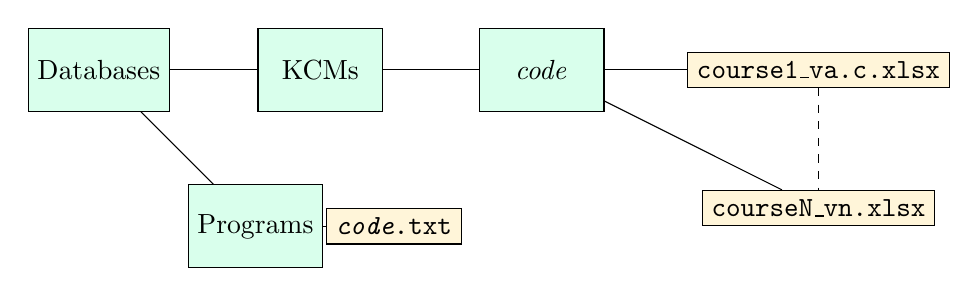
\begin{tikzpicture}[auto]
		\node [block, name=root] {Databases};
		\node [block, name=programs, below right of=root] {Programs};
		\node [file, name=pfile, right of=programs] {\texttt{\textit{code}.txt}};
		\node [block, name=kcms, right of=root] {KCMs};
		\node [block, name=drive, right of=kcms] {\textit{code}};
		\node [file, name=sheet1, right of=drive, node distance=10em] {\texttt{course1\_va.c.xlsx}};
		\node [file, name=sheetN, below of=sheet1] {\texttt{courseN\_vn.xlsx}};
		
		\draw [draw] (root) -- (programs);
		\draw [draw] (root) -- (kcms);
		\draw [draw] (kcms) -- (drive);
		\draw [draw] (programs) -- (pfile);
		\draw [draw] (drive) -- (sheet1);
		\draw [draw] (drive) -- (sheetN);
		\draw [draw, dashed] (sheet1) -- (sheetN);
	\end{tikzpicture}
	\caption{Diagram of the local database of the \ac{KCM} spreadsheet files.}
	\label{fig:dblocal}
\end{figure}

In more details, if one considers the base folder shown in
Figure~\ref{fig:file-structure-base-folder}, one should then enter the
Databases folder (as in Figure~\ref{fig:file-structure-databases-folder}),
and then enter the folder ``KCMs''. For a person that has been analysing
several programs, this ``KCMs'' folder would look like as in
Figure~\ref{fig:file-structure-KCMs-folder} (again, this is an example --
you get an almost empty ``KCMs'' folder when you download the software
suite).

\begin{figure}[!htbp]
	\centering
	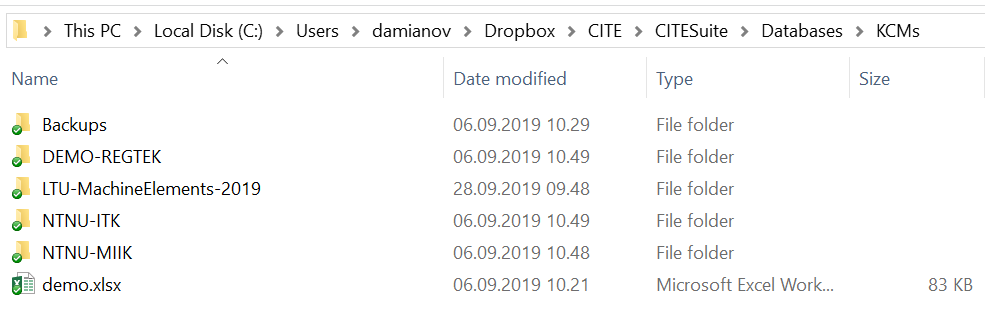
\includegraphics{file-structure-KCMs-folder}
	\caption{Structure of the ``KCMs'' folder for a person that has been analysing several programs.}
	\label{fig:file-structure-KCMs-folder}
\end{figure}

Each folder in the ``KCMs'' folder is then a separate program: in this
sub-folder you shall place your \texttt{.xlsx} files. As an example,
Figure~\ref{fig:file-structure-NTNU-MIIK-folder} shows the content of such a
sub-folder relative to a program in NTNU. Note that one may have different
versions for the same course. Note also that if a \ac{KCM} is not found, the
program will download it from the Internet and copy the downloaded sheet to
its expected location.

\begin{figure}[!htbp]
	\centering
	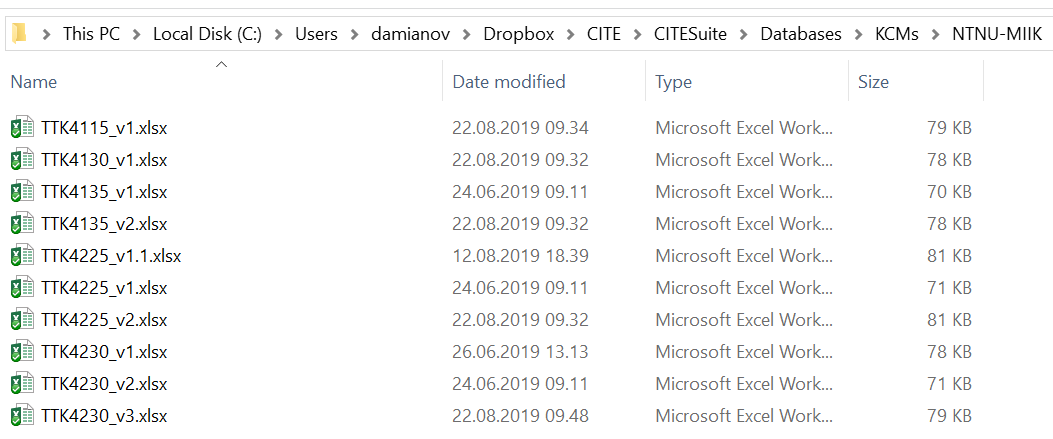
\includegraphics{file-structure-NTNU-MIIK-folder}
	\caption{Contents of a folder that contains the \texttt{.xlsx} files
	describing a given program.}
	\label{fig:file-structure-NTNU-MIIK-folder}
\end{figure}

Note the name formats: the name of each \ac{KCM} file must be on the form
\texttt{coursecode\_v\textit{version}} and have the extension
\texttt{.xlsx}. The \texttt{coursecode} and \textit{version} information
must be the same one that is in the program definition file. The name of the
folder containing the \acp{KCM} of the program must be identical to the name
of the program definition file. The folder itself must be placed in the
\texttt{KCMs} folder.

\subsection{Filling up the various \acp{KCM}}

Each \texttt{.xlsx} spreadsheet capturing a \ac{KCM} has six sheets, described in the following subsections.

\begin{centering}
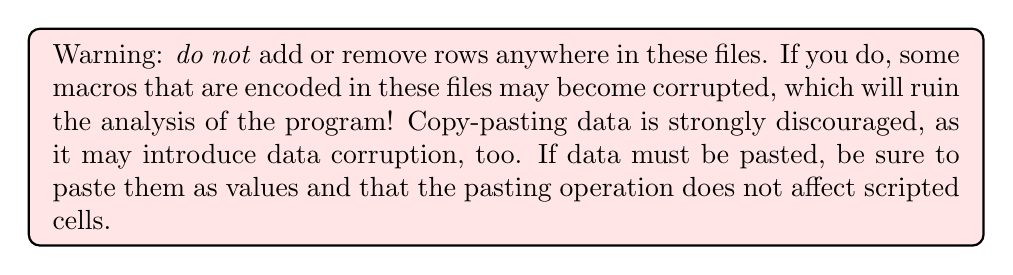
\begin{tikzpicture}
\node [minimum width = \textwidth, rounded corners, draw, thick, fill =
	red!10!white, align = justify, text width = 0.95\textwidth, inner
	sep = 0.2cm]
{Warning: \emph{do not} add or remove rows anywhere in these files. If you
	do, some macros that are encoded in these files may become
	corrupted, which will ruin the analysis of the program! Copy-pasting
	data is strongly discouraged, as it may introduce data corruption,
	too. If data must be pasted, be sure to paste them as values and
	that the pasting operation does not affect scripted cells.};
\end{tikzpicture}
\end{centering}

The template \texttt{.xlsx} has the following colors-scheme:
%
\begin{description}
	\item[gray:] parts that are comments or indications, do not edit
		these;
	\item[pink:] parts that are required (i.e., if you don't fill
		them then you won't get results); 
	\item[yellow:] parts that are optional, but recommended (i.e., if
		you don't fill them then you will get only partial results,
		and not everything that the tool may give you); 
	\item[green:] parts that you should fill if you want to get all the
		results that the suite can compute.
\end{description}
%
Thus: one should fill up at least all the pink parts. Doing the yellow and
green ones will produce more informative results (but of course will also
require more compilation time).


\subsubsection{The course summary sheet}
\label{sssec:the_course_summary_sheet}

The first sheet, called \texttt{course summary}, is a summary of the course and has the following information:

\begin{itemize}

	\itemheader{Prerequisite \acp{KC}}, which is a list of the \acp{KC}
		that are prerequisites for the course, i.e. \acp{KC} that
		students should be familiar with at the beginning of the
		course. See
		Section~\ref{sec:how_to_define_the_knowledge_components_list}
		for a description on how to identify these \acp{KC}. The
		\acp{KCM} supports up to 20 \acp{KC};
	
	\itemheader{Developed \acp{KC}}, which is a list of the \acp{KC}
		that the students should get familiar with as they advance
		through the course.
	
	\itemheader{\acp{TLA}}, which is a list of teaching and learning
		activities (lectures, classes, labs etc.) that occur in the
		course. See Section~\ref{sec:how_to_identify_tla} for a
		description on how to identify these \acp{TLA};
	
	\itemheader{\acp{ILO}}, which is a list of \acp{KC} that the
		students should have acquired after passing the course. See
		Section~\ref{sec:how_to_identify_ilo} for a description on
		how to identify these \acp{ILO};
	
	\itemheader{Starting and ending dates}, which are the dates when the
		course begins and ends, respectively. \textbf{Respect the
		format that is indicated in the \texttt{.xlsx} file};
	
	\itemheader{Taxonomy types}, which is a list of which taxonomy
		types, e.g., ``SOLO'' or ``Bloom'', that are included in
		this \ac{KCM}. If left blank, it defaults to ``SOLO''. See
		Section~\ref{sec:how_to_interpret_and_assign_taxonomy_levels}
		for a description of how to interpret and assign taxonomy
		levels;
	
	\itemheader{Course code}, which is self-explaining. If using a local
		repository, the file name should be equal to this entry.

\end{itemize}


\subsubsection{The developed vs.\ prerequisite KCs sheet}

The second sheet, called ``developed vs.\ prerequisite KCs'', is a
dependency matrix for the developed \acp{KC} versus the prerequisite
\acp{KC} and the developed \acp{KC}. In this matrix, each row is associated
with one of the \acp{KC} that are being developed in the course, and each
column is associated to either a prerequisite \ac{KC} or a developed
\ac{KC}. Assume that \texttt{X} is the row \ac{KC}, and \texttt{Y} is the
column \ac{KC}. Then the content of the cell \texttt{X-Y} shall indicate the
minimum taxonomical knowledge level that the students should have reached
about \texttt{Y} before starting learning \texttt{X} so to be able to learn
\texttt{X} in a satisfactory way. In other words, each entry says how much
(in a taxonomical knowledge way) the column \ac{KC} is instrumental to learn
the row \ac{KC}.

Note that if you did not fill up all 20 slots for the \acp{KC} in the
\texttt{course summary} tab then some rows and/or columns will show a ''0''
in the corresponding cell. This is a result of referencing a blank cell.


\subsubsection{The info on the developed KCs sheet}

The third sheet is a table of the developed \acp{KC} and has the following
information:

\begin{itemize}

	\itemheader{Developed \acp{KC}}, which is the same as in the course
		summary;
	
	\itemheader{Target taxonomy level}, which is the taxonomy level that
		the associated \ac{KC} should be known at by the end of the
		course;
	
	\itemheader{Time spent teaching}, which is the number of hours the
		course invests in teaching the associated \ac{KC};
	
	\itemheader{First lesson}, which is the number of the first teaching
		event when the associated \ac{KC} is taught.

\end{itemize}


\subsubsection{The remaining sheets}

The fourth sheet, called ``KCs vs.\ TLAs'', is similar to the second sheet
in the sense that it also is a dependency matrix. However, the meaning of
the rows and columns indexes is slightly different than before, and
indicates only a \emph{relation}: assume that \texttt{X} is the row
\ac{TLA}, and \texttt{Y} is the column \ac{KC}. Then a nonzero content in
the cell \texttt{X-Y} indicates that \texttt{Y} is either rehearsed or
taught during \texttt{X}. Moreover, the indicated taxonomical knowledge
level indicates at which complexity that rehearsal or teaching happens. In
other words, each entry says how much (in a taxonomical knowledge way) the
column \ac{KC} is rehearsed or taught during the row \ac{TLA}.

The fifth sheet, called ``info on the TLAs'', is similar to the third sheet,
but has information on the \acp{TLA} rather than \acp{KC}. This sheet holds
the following information:

\begin{itemize}

	\itemheader{\ac{TLA}}, which is the same as in the course summary;
	
	\itemheader{Time spent on activity}, which is the number of hours
		this course spends on the associated \ac{TLA};
	
	\itemheader{When the \ac{TLA} starts}, which is the number of the
		teaching event when the course starts hosting the associated
		\ac{TLA};
	
	\itemheader{When the \ac{TLA} ends}, which is the number of the
		teaching event when the course stops hosting the associated
		\ac{TLA}.

\end{itemize}

The sixth sheet, called ``developed KCs vs.\ ILOs'', is equivalent to the
fourth sheet. This time, though, each entry says how much (in a taxonomical
knowledge way) the column \ac{KC} is needed to reach the row \ac{ILO}.

\subsection{Summary of the procedure}

To summarize, to create a database that can be analysed through the COnCUR
one should follow these macro-steps:

\begin{enumerate}

	\itemheader{Create the program definition file}. This text document
		holds course codes, version numbers and links to these
		\acp{KCM} if they are on the Internet.
	
	\itemheader{Place the \acp{KCM} in the correct location}. If
		downloading the files over Internet, ensure that the links
		in the program definition file point to the correct URLs. If
		using a local repository, ensure that the \acp{KCM} are
		placed in the correct folder and named correctly.

\end{enumerate}


\section{Analysing the data}
\label{sec:analysing_the_data}

\subsection{Launching Matlab}

Note that to launch the CITE app below one needs Matlab 2019a or a higher version. The KCM analysis part, instead, requires Matlab 2018a or a higher version.

Once Matlab is launched, one shall change the directory in the command window to the folder "Scripts" (cf.\ Figure~\ref{fig:file-structure-base-folder}). Once there, execute \texttt{main.m}.

\subsection{The initial prompt}

Launching \texttt{main.m} will initially produce a series of debug messages, and then a prompt like the one in Figure~\ref{fig:main-menu}.

\begin{figure}[!htbp]
	\centering
	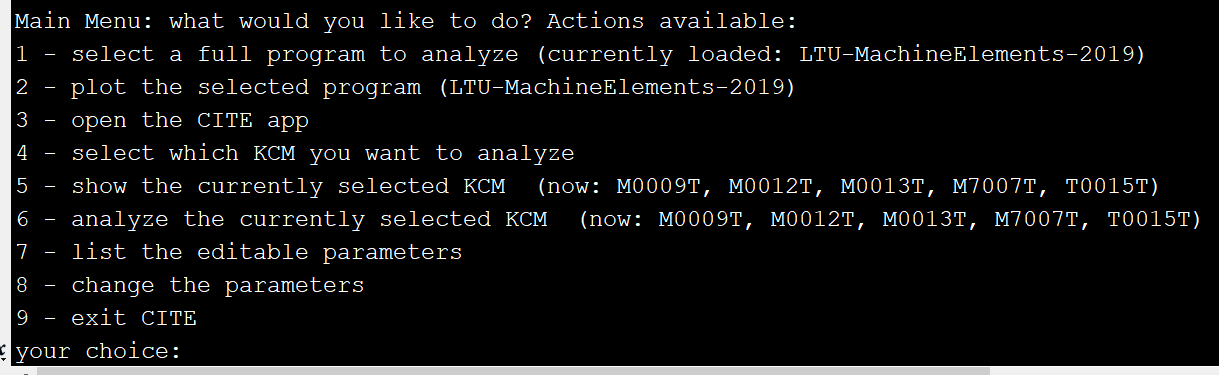
\includegraphics[width = 0.8\textwidth]{main-menu}
	\caption{Main menu that one obtains by launching \texttt{main.m}.}
	\label{fig:main-menu}
\end{figure}

The most interesting (and not self-explaining) items are:
%
\begin{itemize}
	\item ``plot the selected program'', that will produce a figure that summarizes which course connects with which other in terms of \acp{KC}. Note that the suite will assign all the prerequisite \acp{KC} that are not taught by any course to an artificial ``prerequisites'' course. Note also that the plot is explorable - in the sense that clicking on the various arrows will expand which \acp{KC} form the connections;
	\item ``open the CITE app'' - for this item see Section~\ref{ssec:the_cite_app};
	\item ``analyse the currently selected KCM'' - for this item see Section~\ref{ssec:the_kcm_analysis_prompt}.
\end{itemize}


\subsection{The KCM analysis prompt}
\label{ssec:the_kcm_analysis_prompt}

Selecting to analyse the currently selected KCM will produce a prompt like the one in Figure~\ref{fig:KCM-analysis-menu}.

\begin{figure}[!htbp]
	\centering
	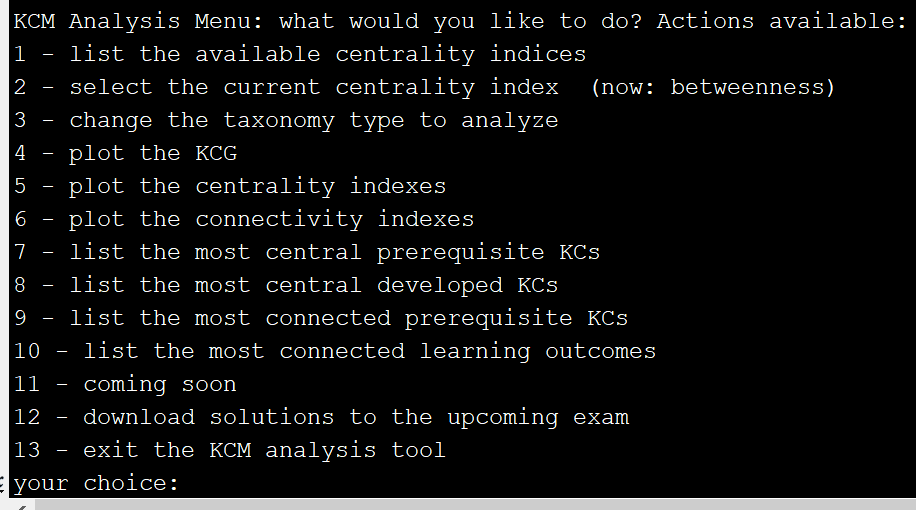
\includegraphics[width = 0.8\textwidth]{KCM-analysis-menu}
	\caption{Menu that one obtains by launching an analysis of the currently selected KCM.}
	\label{fig:KCM-analysis-menu}
\end{figure}

The most interesting (and not self-explaining) items are:
%
\begin{itemize}
	\item ``plot the KCG'', that will open the CITE app (thus check Section~\ref{ssec:the_cite_app} for this item);
	\item ``plot the centrality indexes'', that will produce a figure that should be interpreted as suggested in Section~\ref{sec:interpreting_the_results}.
\end{itemize}

\subsection{The CITE app}
\label{ssec:the_cite_app}

Once the app is launched, you will get a blank graph plot, and a list of courses on the right. Selecting the desired courses with the mouse (shift+click) and then pressing the ``Plot'' button will produce an other explorable plot. Here clicking on the various nodes will highlight connections. Different colors are also placeholders for different taxonomical levels. Clicking the ``Show Structural Problems'' item will moreover highlight structural issues in the \ac{KCG}, that may be either of a temporal structure (i.e., a course assumes that a prerequisite \ac{KC} has been taught, but it has actually been taught at a later course) or taxonomical level structure (i.e., one assumes that a prerequisite has been previously taught at a certain level, but actually it has been taught at a lower level).



\section{Interpreting the results}
\label{sec:interpreting_the_results}

\subsection{Interpreting the centrality indexes}

\begin{description}

	\item[out degree:] when considering a course, a high out-degree
		indicates that this course exposes students to \acp{KC} that
		are likely being introductory or instrumental to build a
		framework later on. This means that assessments in courses
		that have high out degrees correspond to "baseline
		assessments", i.e., evaluations of students' initial
		knowledge. Similar concepts apply to a \ac{KC}: a high out
		degree would imply that this \acp{KC} likely represents
		baseline knowledge;

	\item[in degree:] when considering a course, a high in-degree
		indicates that this course is the destination of the
		learning efforts. From a pedagogical perspective this
		indirectly indicates courses where it is important to engage
		students with active and higher-level learning activities.
		Assessments on these courses are a sort of "final
		assessments" for the program. Similar concepts apply to a
		\ac{KC};

	\item[betweenness:] when considering a course, a high betweenness
		indicates that this course serves as a key link between
		different clusters of courses or \acp{KC} in a program. This
		indicates that they serve as a bridge; for this reason
		assessments on courses with high betweenness serve both the
		purposes described above, i.e., as evaluations of students'
		initial knowledge for the next "cluster" of courses, and of
		students final knowledge for the previous "cluster" of
		courses. Similar concepts apply to a \ac{KC};

	\item[eigenvector centrality:] in graph theory, the eigenvector
		centrality measures the influence of a node in a network in
		a similar way that the Google pagerank algorithm works: if a
		node is pointed to by many nodes which also have high
		eigenvector centrality then that node will have high
		eigenvector centrality. In a sense, the links of a node with
		higher eigenvector centrality are more influential than the
		links of a node with a lower centrality index. When
		considering a course, an interpretation of this index is in
		terms of "how much this course serves as a support and
		reinforcement for other courses". Assessments on courses
		with high eigenvector centrality indexes serve as
		complementary assessments for other courses;

% 	\item[clustering coefficient:] Vectors with a high clustering coefficient are the ones most likely to efficiently enact change to the adjacent vectors. The clustering coefficient is useful in finding the course that can most efficiently implement change into adjacent courses. This is relevant because all assessment schemes require a feedback mechanism to modify the curriculum when the assessment data indicate a problem. The quicker this change can be incorporated into the curriculum, the sooner improved results will (hopefully) occur. Those courses with the highest clustering coefficient are the ones best suited for quick, efficient implementation.

	\item[incloseness:] yet to be interpreted
		% Something about being close to the predecessors of the
		% \ac{KC}.

	\item[outcloseness:] yet to be interpreted
		% Like incloseness, but for successors.

	\item[authorities:] yet to be interpreted

	\item[hubs:] yet to be interpreted

\end{description}


% \subsection{The connectivity indexes graph}
% 
% \emph{\ldots to be done \ldots}


% \subsection{Interpreting the \ac{KCG}}





\appendix
\newpage

\section{Lexicon}
\label{sec:lexicon}

\begin{description}

	\item[Bloom's taxonomy:] set of hierarchical models useful to classify learning objectives into levels of complexity and specificity. The models capture these different levels in different domains - namely cognitive, affective and sensory. For engineering and natural sciences purposes the most important is likely the cognitive one, whose levels are reported in Table~\ref{tab:blooms-taxonomy};

		\begin{table}[!htbp]
			\centering
			\begin{tabular}{|llp{0.7\textwidth}|}
				\hline
				1 & \emph{Remember} & be able to recognize or remember facts, terms, basic concepts, or answers without necessarily understanding what they mean \\
				2 & \emph{Understand} & be able to organize, compare, translate, interpret, give descriptions, and state the main ideas \\
				3 & \emph{Apply} & be able to use prior knowledge to solve problems, identify connections and relationships and how they apply in new situations \\
				4 & \emph{Analyze} & be able to break information into component parts, determine how the parts relate to one another, identify motives or causes, make inferences, and find evidence to support generalizations \\
				5 & \emph{Evaluate} & be able to present and defend opinions by making judgments about information, the validity of ideas, or quality of work based on a set of criteria \\
				6 & \emph{Create} & be able to build a structure or pattern from diverse elements and to put parts together to form a whole \\
				\hline
			\end{tabular}
			\caption{Summary of the knowledge levels defined in Bloom's taxonomy~\cite{bloom1956taxonomy}.}
			\label{tab:blooms-taxonomy}
		\end{table}

	\item[\acfp{ILO}:] what students should know or be able to do at the end of the course that they couldn't do before. They should be about students performance. Typical verbs used to describe \acp{ILO} are: ``Memorize, identify, recognize, define, find, classify, describe, list, discuss, select, compute, analyse, explain, compare, construct, review, solve, prove,'' etc;

	\item[\acfp{KC}:] acquirable units of cognitive functions. They can be facts, concepts, procedures, etc. Importantly, a \ac{KC} must have the quality that it is possible to design tests that can show whether a student has acquired that \ac{KC} or not. \emph{If one defines something for which one cannot test whether a student acquired that thing or not, then that thing is not a \ac{KC}.} Specially important cases of \acp{KC} in engineering and natural sciences education are \emph{facts}, \emph{procedures} and \emph{concepts}. These correspond to mental representations, abstract objects or abilities that make up the fundamental building blocks of thoughts and beliefs, plus instructions, recipes, or sets of commands that show how to achieve some result, such as to prepare or make something;

	\item[\ac{SOLO} taxonomy:] a taxonomy that describes levels of increasing complexity in students' understanding of subjects. In practice, a way of classifying educational learning objectives into levels of complexity and specificity. A graphical illustration of the SOLO taxonomy is given in Figure~\ref{fig:SOLO-taxonomy}. A video explaining what the levels mean using LEGOs as an example can be found searching ''SOLO taxonomy using LEGO'' in youtube.

		\begin{figure}[!htbp]
			\centering
			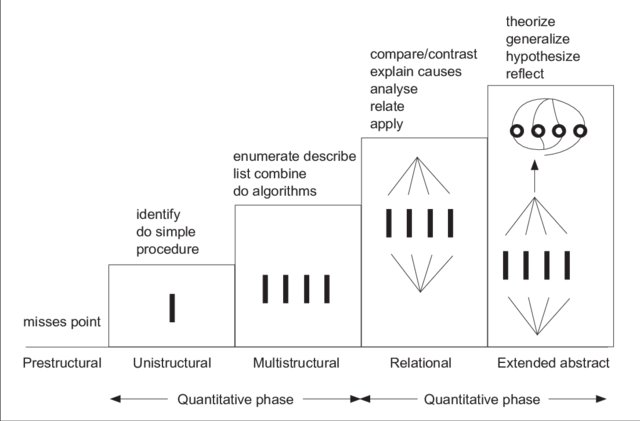
\includegraphics[width = 0.8\textwidth]{SOLO-Taxonomy}
			\caption{Graphical representation of the \ac{SOLO} taxonomy as proposed in~\cite{biggs1982evaluation}.}
			\label{fig:SOLO-taxonomy}
		\end{figure}

	\item[taxonomy:] (i.e., a set of ordered labels) 

	\item[\acfp{TLA}:] the work that is done in and out of the class in relation to the course, e.g., seminars, lectures, labs, etc. See \url{https://www.uwc.ac.za/TandL/Pages/TandL-Activities.aspx} for some more examples; 

\end{description} 


\section{How to define the knowledge components list}
\label{sec:how_to_define_the_knowledge_components_list}

To be done.


\section{How to interpret and assign taxonomy levels}
\label{sec:how_to_interpret_and_assign_taxonomy_levels}

To be done.


\section{How to identify \acp{ILO}}
\label{sec:how_to_identify_ilo}

To be done.


\section{How to identify \acp{TLA}}
\label{sec:how_to_identify_tla}

To be done.


\section{Debugging}
\label{sec:debugging}

\begin{itemize}
	
	\item Be sure that each \texttt{.xlsx} has 24 rows in the 'course summary tab', and that the last two rows are 'course starting date' and 'course ending date';

	\item put a zero in the A1 cell of the non-first-sheet of the various \ac{KCM} files. This serves as an ``anchor'' for Matlab;

	\item each column in the program definition file has to be separated by \textbf{one} tab (see Section~\ref{creating_the_database}).

\end{itemize}




\section{Bibliography}
\bibliographystyle{plain}
\bibliography{bibliography} % bibliography.bib

\end{document}

Versions:
0.1: initial release

